\chapter{Datapath}
Now we can take a closer look at the implementation of RISC-V. 

\section{Overview}
In the implementation, we use the program counter (PC). After supplying the instruction address and fetching the instruction from memory, we update the PC. Then, we decode the instruction and execute it.

There are two types of functional units (logic elements). The first type is combinational (combinational elements), which operate on data values. The output of these functional units depends only on the current input, meaning there is no internal storage. The second type includes elements that contain state, called state elements. These elements have internal storage, which characterizes a computer. For example, instruction memory, register files, and data memory are sequential (state elements), while the ALU is combinational.

\begin{remark}
  In instruction memory, instructions are placed one by one. In register files, there are 32 lines, and we only need 5 bits in the instruction to indicate the register file address.
\end{remark}

To fetch instructions, the processor first reads the instructions from the instruction memory, then updates the PC to the address of the next instruction. The PC is updated every clock cycle (typically \(\text{PC} = \text{PC} + 4\) by default), and the instruction memory is read every clock cycle.

Note that the clock is edge-triggered, so the PC is updated only on the rising or falling edge of the clock.

After the instructions are read, the processor decodes them. The fetched instruction's opcode and function field bits are sent to the control unit, which then generates control signals used in the future datapath. Next, two values are read from the Register File, with the register addresses contained in the instruction. 

Regardless of whether the values are actually used, the Register File's read ports are active for all instructions during the decode cycle. In case the instruction requires values from the Register File, it reads the two source operands by default. 

All instructions, except \verb|j|, use the ALU after reading from the register. For memory-reference instructions, the ALU is used to compute addresses; for arithmetic instructions, the ALU performs the required arithmetic; for control instructions, the ALU computes branch conditions.

\section{Operations}
\subsection{R Format Operations}
\begin{center}
\begin{bytefield}[leftcurly=., leftcurlyspace=0pt, bitwidth=12pt]{32}
\bitheader[endianness=big]{31, 25, 24, 20, 19, 15, 14, 12, 11, 7, 6, 0} \\
\begin{leftwordgroup}{\makebox[\widthof{R-Type\ }][r]{R-Type\ }}
\bitbox{7}{funct7} & \bitbox{5}{rs2} & \bitbox{5}{rs1} & \bitbox{3}{funct3} & \bitbox{5}{rd} & \bitbox{7}{opcode}
\end{leftwordgroup}\\
\end{bytefield}
\end{center}

R-type instructions perform operations on values in \verb|rs1| and \verb|rs2|, then store the result back into the Register File. Note that the Register File is not written every cycle, so a write control signal is needed for the Register File.

\subsection{I and S Format Operations}
\begin{center}
\begin{bytefield}[leftcurly=., leftcurlyspace=0pt, bitwidth=12pt]{32}
\bitheader[endianness=big]{31, 20, 19, 15, 14, 12, 11, 7, 6, 0} \\
\begin{leftwordgroup}{\makebox[\widthof{I-Type\ }][r]{I-Type\ }}
\bitbox{12}{imm[11:0]} & \bitbox{5}{rs1} & \bitbox{3}{funct3} & \bitbox{5}{rd} & \bitbox{7}{opcode}
\end{leftwordgroup}\\
\end{bytefield}
    
\begin{bytefield}[leftcurly=., leftcurlyspace=0pt, bitwidth=12pt]{32}
\bitheader[endianness=big]{31, 25, 24, 20, 19, 15, 14, 12, 11, 7, 6, 0} \\
\begin{leftwordgroup}{\makebox[\widthof{S-Type\ }][r]{S-Type\ }}
\bitbox{7}{imm[11:5]} & \bitbox{5}{rs2} & \bitbox{5}{rs1} & \bitbox{3}{funct3} & \bitbox{5}{imm[4:0]} & \bitbox{7}{opcode}
\end{leftwordgroup}\\
\end{bytefield}
\end{center}

For load and store operations, the memory address is computed by adding the base register to the 12-bit signed offset field in the instruction (\verb|imm[] + rs1|). The base register is read from the Register File during decode, and the offset value in the lower 12 bits of the instruction must be sign-extended to create a 32-bit signed value.

For store instructions, the value is read from the Register File during decode and written into the Data Memory. For load instructions, the value is read from the Data Memory and then stored into the Register File.

Also, note that the \verb|lw| and \verb|sw| instructions access data memory, not instruction memory.

\begin{center}
  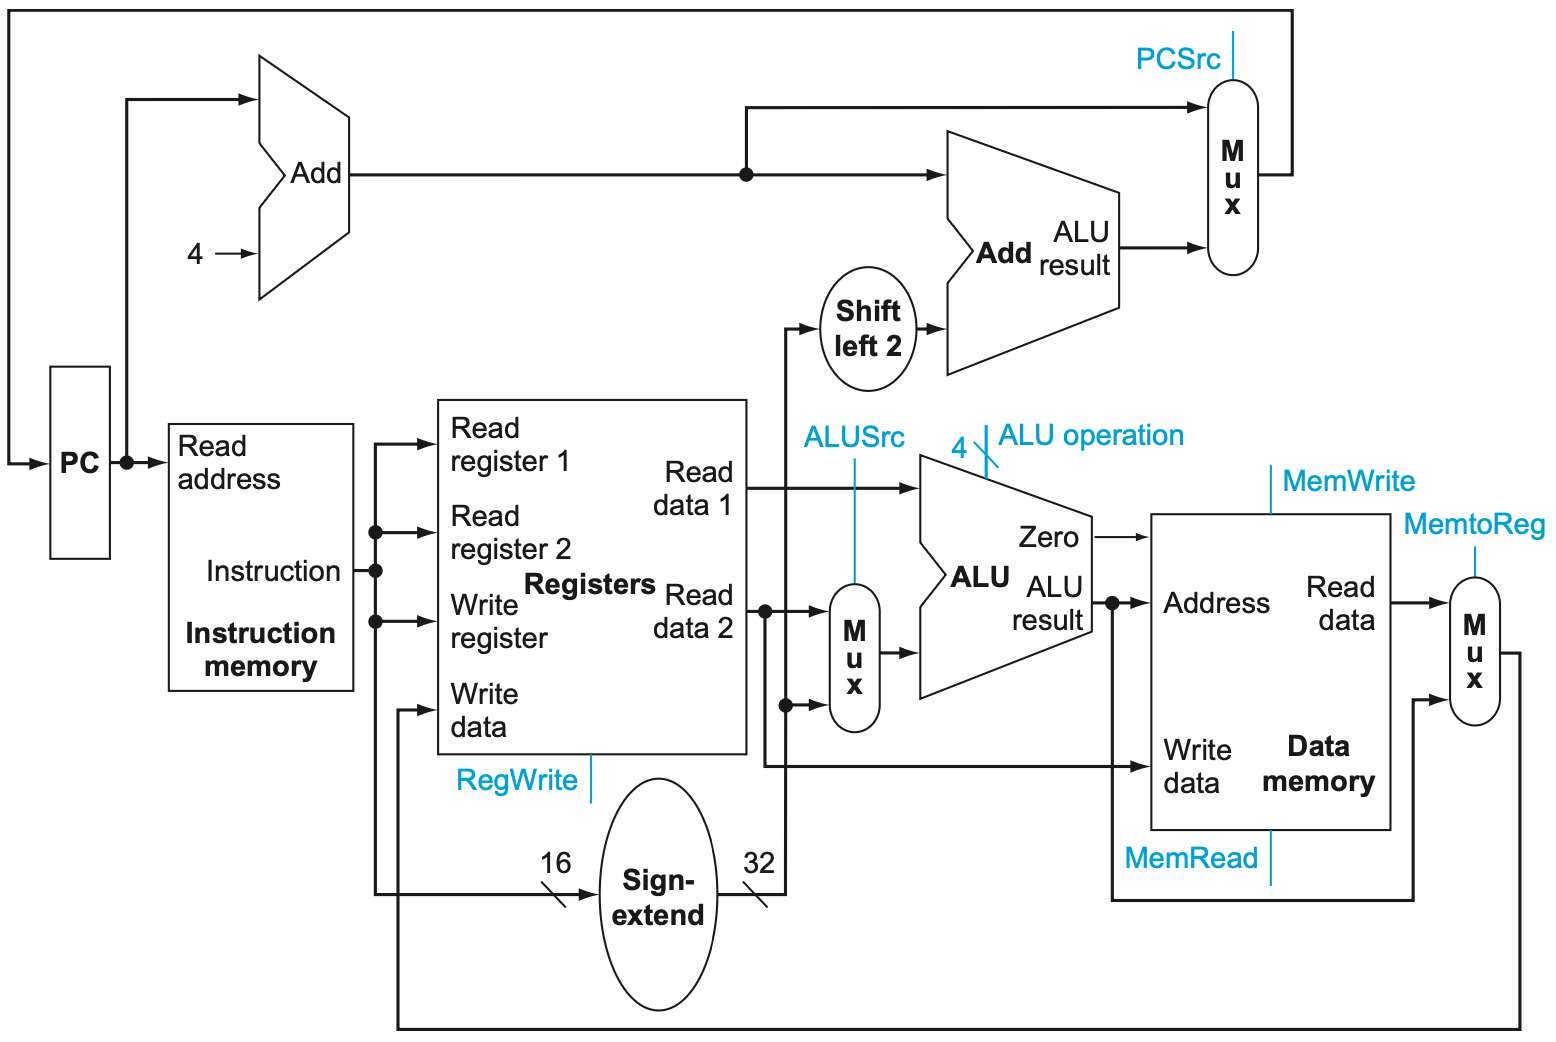
\includegraphics[width=0.5\textwidth]{Figure/ISformat.png}
\end{center}

As shown above, after decoding, the sign is extended in the lower part. Above is the clock for the PC value, which executes the branch instruction. In the rightmost mux, it selects the source. It is activated only for \verb|lw| instructions. Additionally, only for \verb|sw|, the MemWrite signal will be 1 (High), which activates the write data port.

\newpage
\subsection{B Format Operations}
\begin{center}
\begin{bytefield}[leftcurly=., leftcurlyspace=0pt, bitwidth=12pt]{32}
\bitheader[endianness=big]{31, 30, 25, 24, 20, 19, 15, 14, 12, 11, 8, 7, 6, 0} \\
\begin{leftwordgroup}{\makebox[\widthof{B-Type\ }][r]{B-Type\ }}
\bitbox{7}{imm[12|10:5]} & \bitbox{5}{rs2} & \bitbox{5}{rs1} &\bitbox{3}{funct3} & \bitbox{5}{imm[4:1|11]} & \bitbox{7}{opcode}
\end{leftwordgroup}\\
\end{bytefield}
\end{center}

For branch operations, it compares the operands read from the Register File during decode for equality. The 12-bit B-immediate encodes signed offsets in multiples of one byte. It is sign-extended and added to the address of the branch instruction to give the target address.

\subsection{J Format Operations}
\begin{center}
\begin{bytefield}[leftcurly=., leftcurlyspace=0pt, bitwidth=12pt]{32}
\bitheader[endianness=big]{31, 30, 21, 20, 19, 12, 11, 7, 6, 0} \\
\begin{leftwordgroup}{\makebox[\widthof{J-Type\ }][r]{J-Type\ }}
\bitbox{20}{imm[20|10:1|11|19:12]} & \bitbox{5}{rd} & \bitbox{7}{opcode}
\end{leftwordgroup}\\
\end{bytefield}
\end{center}

The J-immediate encodes a signed offset in multiples of 2 bytes. The offset is sign-extended and added to the address of the jump instruction to form the jump target address. Since \verb|imm[0]| is always 0, we don't have it in the instruction. 

The partition of \verb|imm| field is designed to align the \verb|imm| bits better with other instruction types, enabling a more efficient implementation of control units.

\section{Datapath}
By assemble the above datapathn elements, add control lines and desgin the control path, we can create a signle datapath. 

We need to fetch, decode, and execute each instruction in one clock cycle, which is called the single-cycle design. No datapath resource can be used more than once per instruction, so some components must be duplicated. Additionally, multiplexers are needed at the input of the shared elements with control lines to perform the selection, allowing datapath elements to be shared between two different instructions.

\begin{center}
  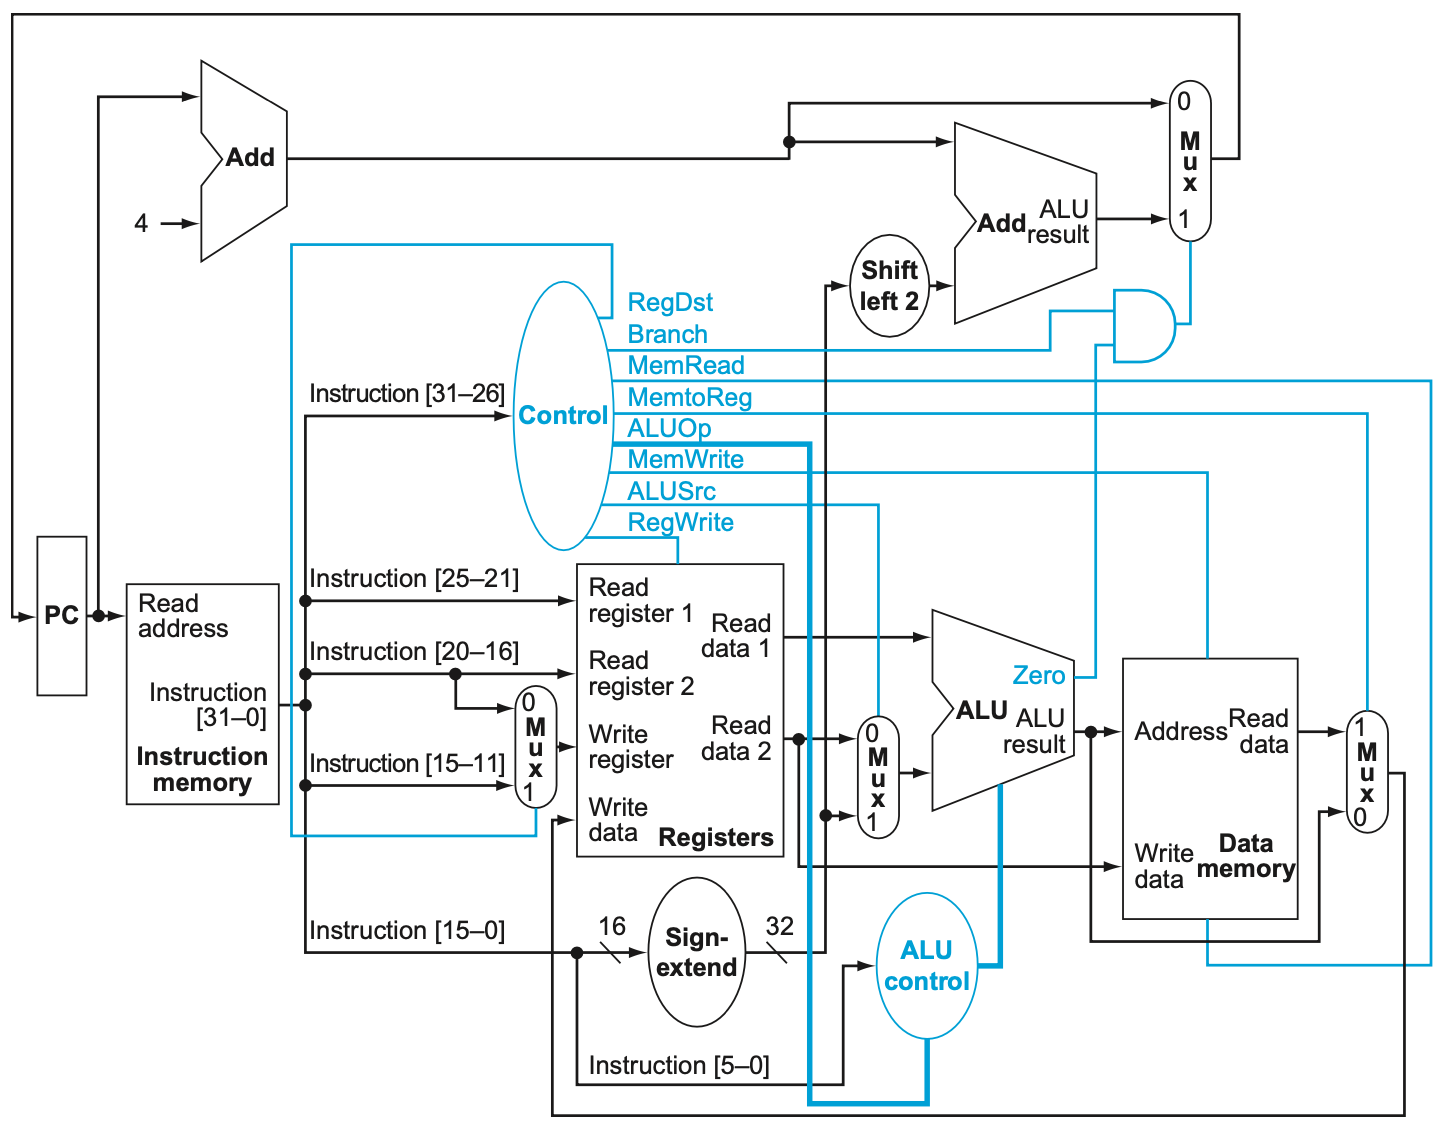
\includegraphics[width=0.8\textwidth]{Figure/Datapath.png}
\end{center}

Here, the MUX before the ALU determines the second ALU operand, and the MUX after the Data Memory decides whether to feed memory data to the register file. The system clock is edge-triggered and is determined by the length of the longest path. The ALU is used to compute the branch instruction, and its output can replace the PC when needed.

Memory and Register File reads are combinational. By using write signals along with the clock edge, we determine when to write to the sequential elements, such as the PC or Register File.

By adding the control as shown above, we can select the operations to perform, control the flow of data, and direct the information that comes from the 32-bit instruction.

\begin{remark}
  The instruction is decoded in the path between the Instruction Memory and Register File.
\end{remark}

For different operations, the control signals vary.
\begin{table}[H]
  \centering
  \begin{tabular}{c|c|c|c|c}
      \toprule
       & \verb|add| & \verb|lw| & \verb|sw| & \verb|beq|  \\
    \midrule
      MUX after Reg & 0 & 1 & 1 & 0  \\
      MUX after DataMem & 0 & 1 & / & /  \\
      MUX after Add & 0 & 0 & 0 & /  \\
      RegWrite & 1 & 1 & 0 & 0  \\
      MemWrite & 0 & 0 & 1 & 0  \\
      MemRead & 0 & 1 & 0 & 0  \\
      \bottomrule
  \end{tabular}
\end{table}

When the MUX after Add \(= 0\), the PC is updated as \(\text{PC} += 4\). Both ALU inputs are from the Register File.
